\documentclass{beamer}
%
% Choose how your presentation looks.
%
% For more themes, color themes and font themes, see:
% http://deic.uab.es/~iblanes/beamer_gallery/index_by_theme.html
%
\mode<presentation>
{
  \usetheme{default}      % or try Darmstadt, Madrid, Warsaw, ...
  \usecolortheme{default}
  \usepackage{beamerthemesplit}% or try albatross, beaver, crane, ...
  \usefonttheme{default}  % or try serif, structurebold, ...
  \setbeamertemplate{navigation symbols}{}
  \setbeamertemplate{caption}[numbered]
  \usepackage{circuitikz}
  \usepackage{tikz}
} 

\usepackage[english]{babel}
\usepackage[utf8x]{inputenc}
\usepackage{amsmath}

% \logo{\vspace{-0.3cm}\includegraphics[height=0.75cm]{D0.png}}
\title[ \hspace{0.5cm}\insertframenumber/\inserttotalframenumber]{Attention Is All You Need}
\author{Shah Jainam EE21B122 \& Ayush Ranjan EE21B026}
\institute{Indian Institute of Technology \\ Madras}
\date{25-04-2025}

\begin{document}

\begin{frame}
  \titlepage
\end{frame}

% Uncomment these lines for an automatically generated outline.
%\begin{frame}{Outline}
%  \tableofcontents
%\end{frame}

%\section{Introduction}

\begin{frame}{Machine Translation Problem}

\begin{itemize}
    \item The motivation for this paper is to solve the problem of text translation.
    \item  Recurrent neural networks, long short-term memory \footnote{Sepp Hochreiter and Jürgen Schmidhuber,1997} and gated recurrent \footnote{Junyoung Chung, Çaglar Gülçehre, Kyunghyun Cho, and Yoshua Bengio} neural networks in particular, have been firmly established as state of the art approaches in sequence modeling and transduction problems such as language modeling and machine translation
\end{itemize}

\begin{figure}[htbp]
    \centering
    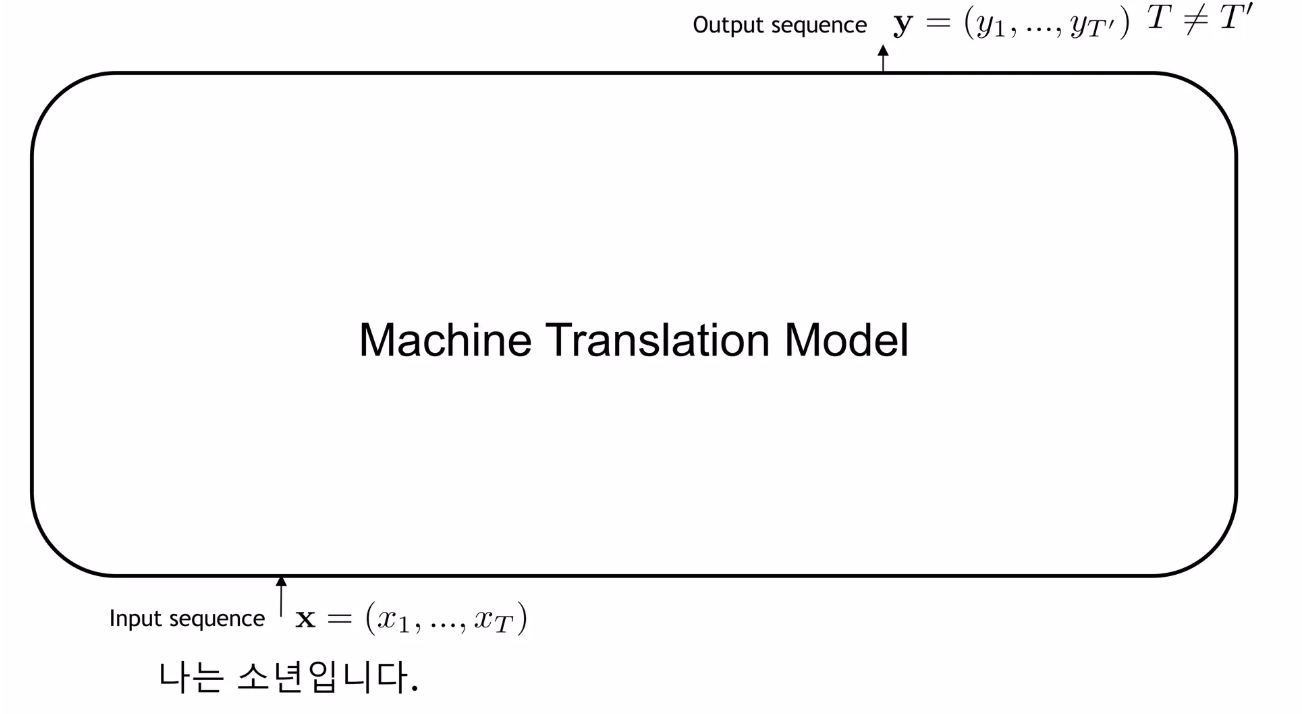
\includegraphics[width=0.6\linewidth]{f1.png}
    \label{fig:enter-label}
\end{figure}
\end{frame}

\begin{frame}{RNN Encoder-Decoder Model}
\begin{figure}
    \centering
    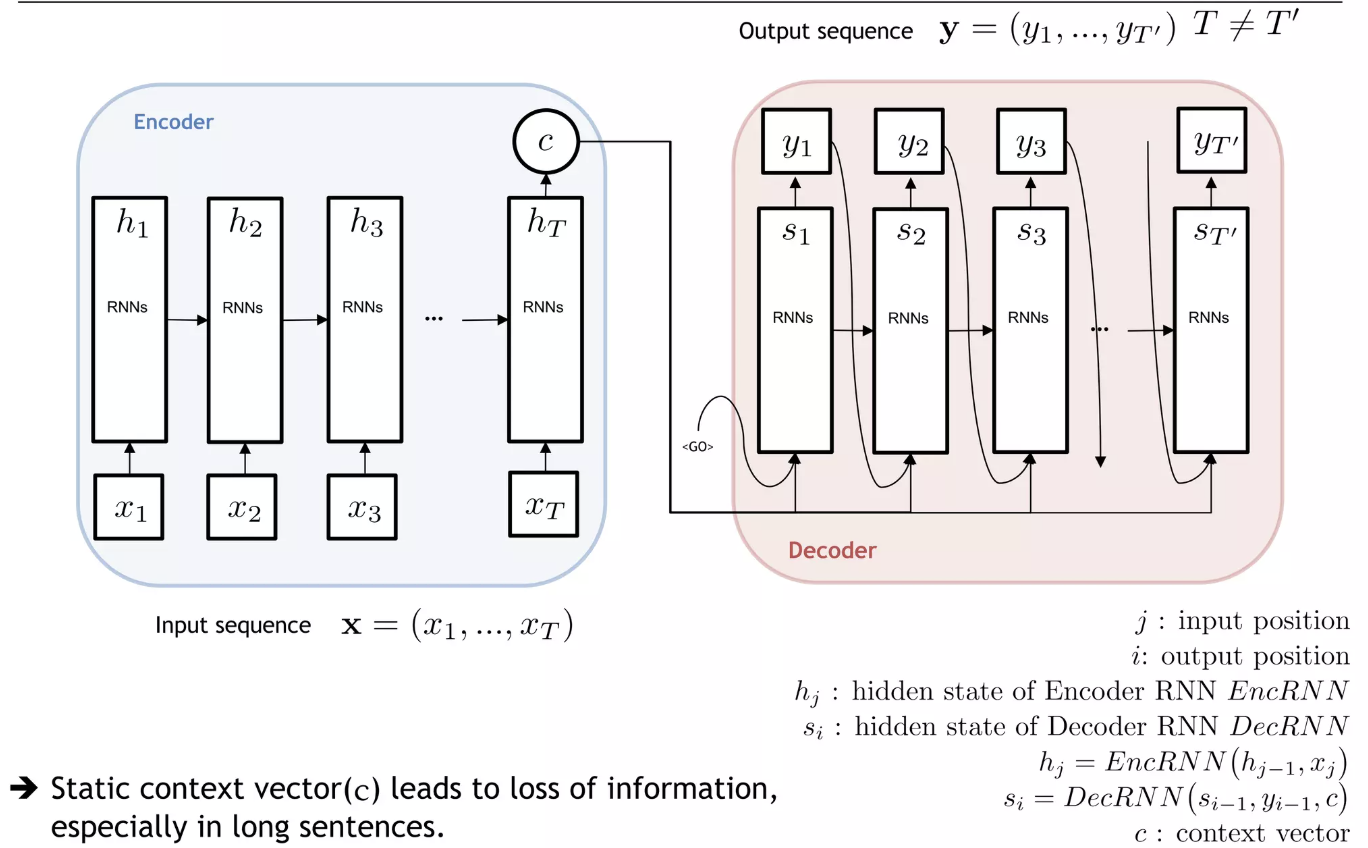
\includegraphics[width=1\linewidth]{f2.png}
    \label{fig:enter-label}
\end{figure}
    
\end{frame}

\begin{frame}{Limits of Recurrent Neural Network}

\begin{itemize}
    \item RNN generates each hidden state in series.
        \begin{itemize}
            \item This sequential nature increases the training time by a large margin.
        \end{itemize}
    \item RNN has long term dependency problems.
        \begin{itemize}
            \item It's hard to remember long term context information.
            \item Attempts to add attention mechanism to RNN have been tried. \footnote{Neural Machine Translation by Jointly Learning to Align and Translate Dzmitry Bahdanau, Kyunghyun Cho, Yoshua Bengio}
        \end{itemize}
    \item RNN can see one word at a time
        \begin{itemize}
            \item CNN can see more than one at a time.
        \end{itemize}
\end{itemize}
\end{frame}

\begin{frame}{Transformers}
\begin{itemize}
    \item Transformers were developed to solve the problem of machine translation and sequence transduction, or neural machine translation, but they can do so much more.
\end{itemize}

\begin{columns}
  % Left Column for Image
  \column{0.4\textwidth}
  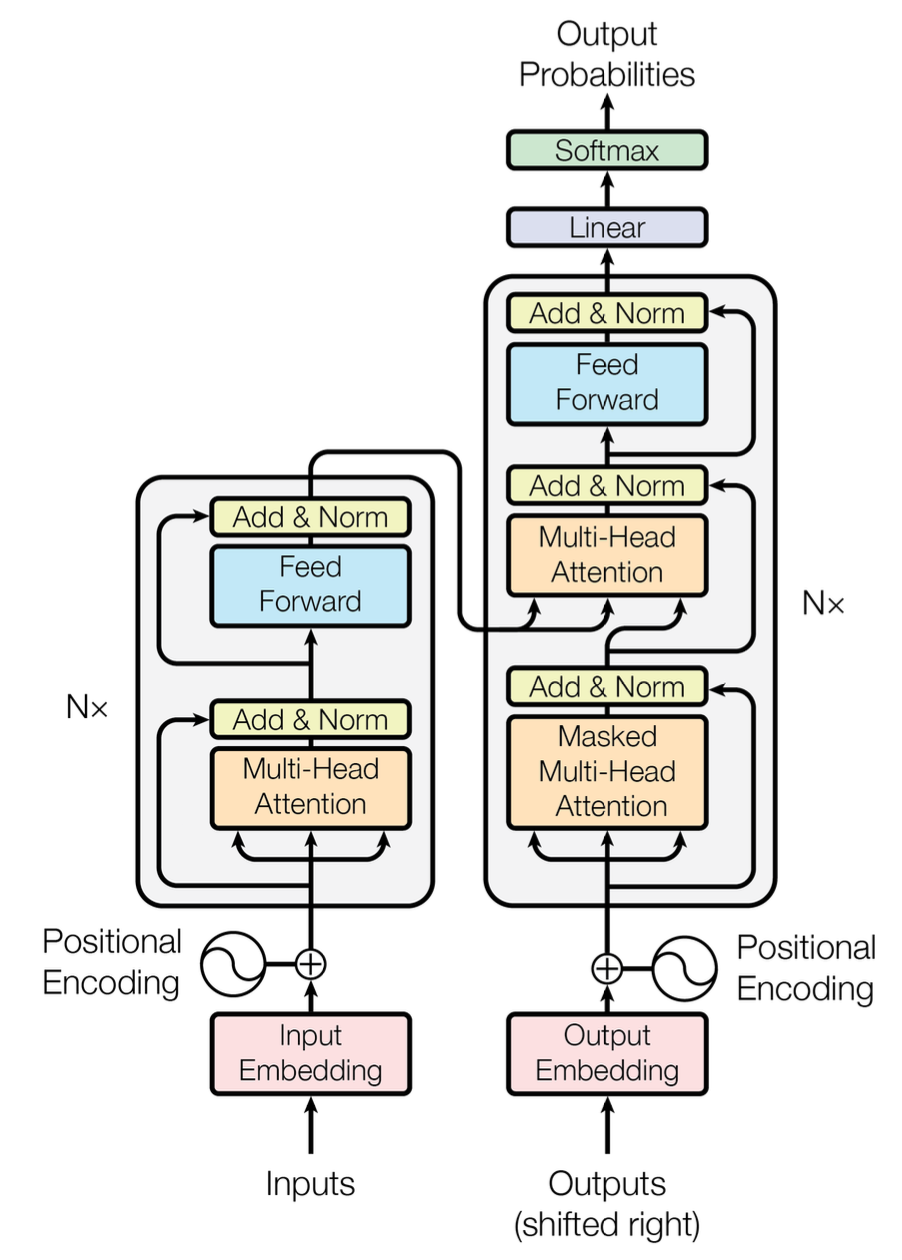
\includegraphics[width=1\linewidth]{f3.png} % Replace with your image filename

  % Right Column for Text
  \column{0.6\textwidth}
      \begin{itemize}
          \item Great performance in computer vision like ViT (Dosovitskiy, 2020)
          \item Image Classification (CoCa Transformer)
          \item Semantic Segmentation (e.g., FD-SwinV2-GTransformer)
          \item Object Detection (e.g., FD-SwinV2-GTransformer)
      \end{itemize}

\end{columns}
\end{frame}

\begin{frame}{Full Architecture of Transformer.}
    \begin{figure}
        \centering
        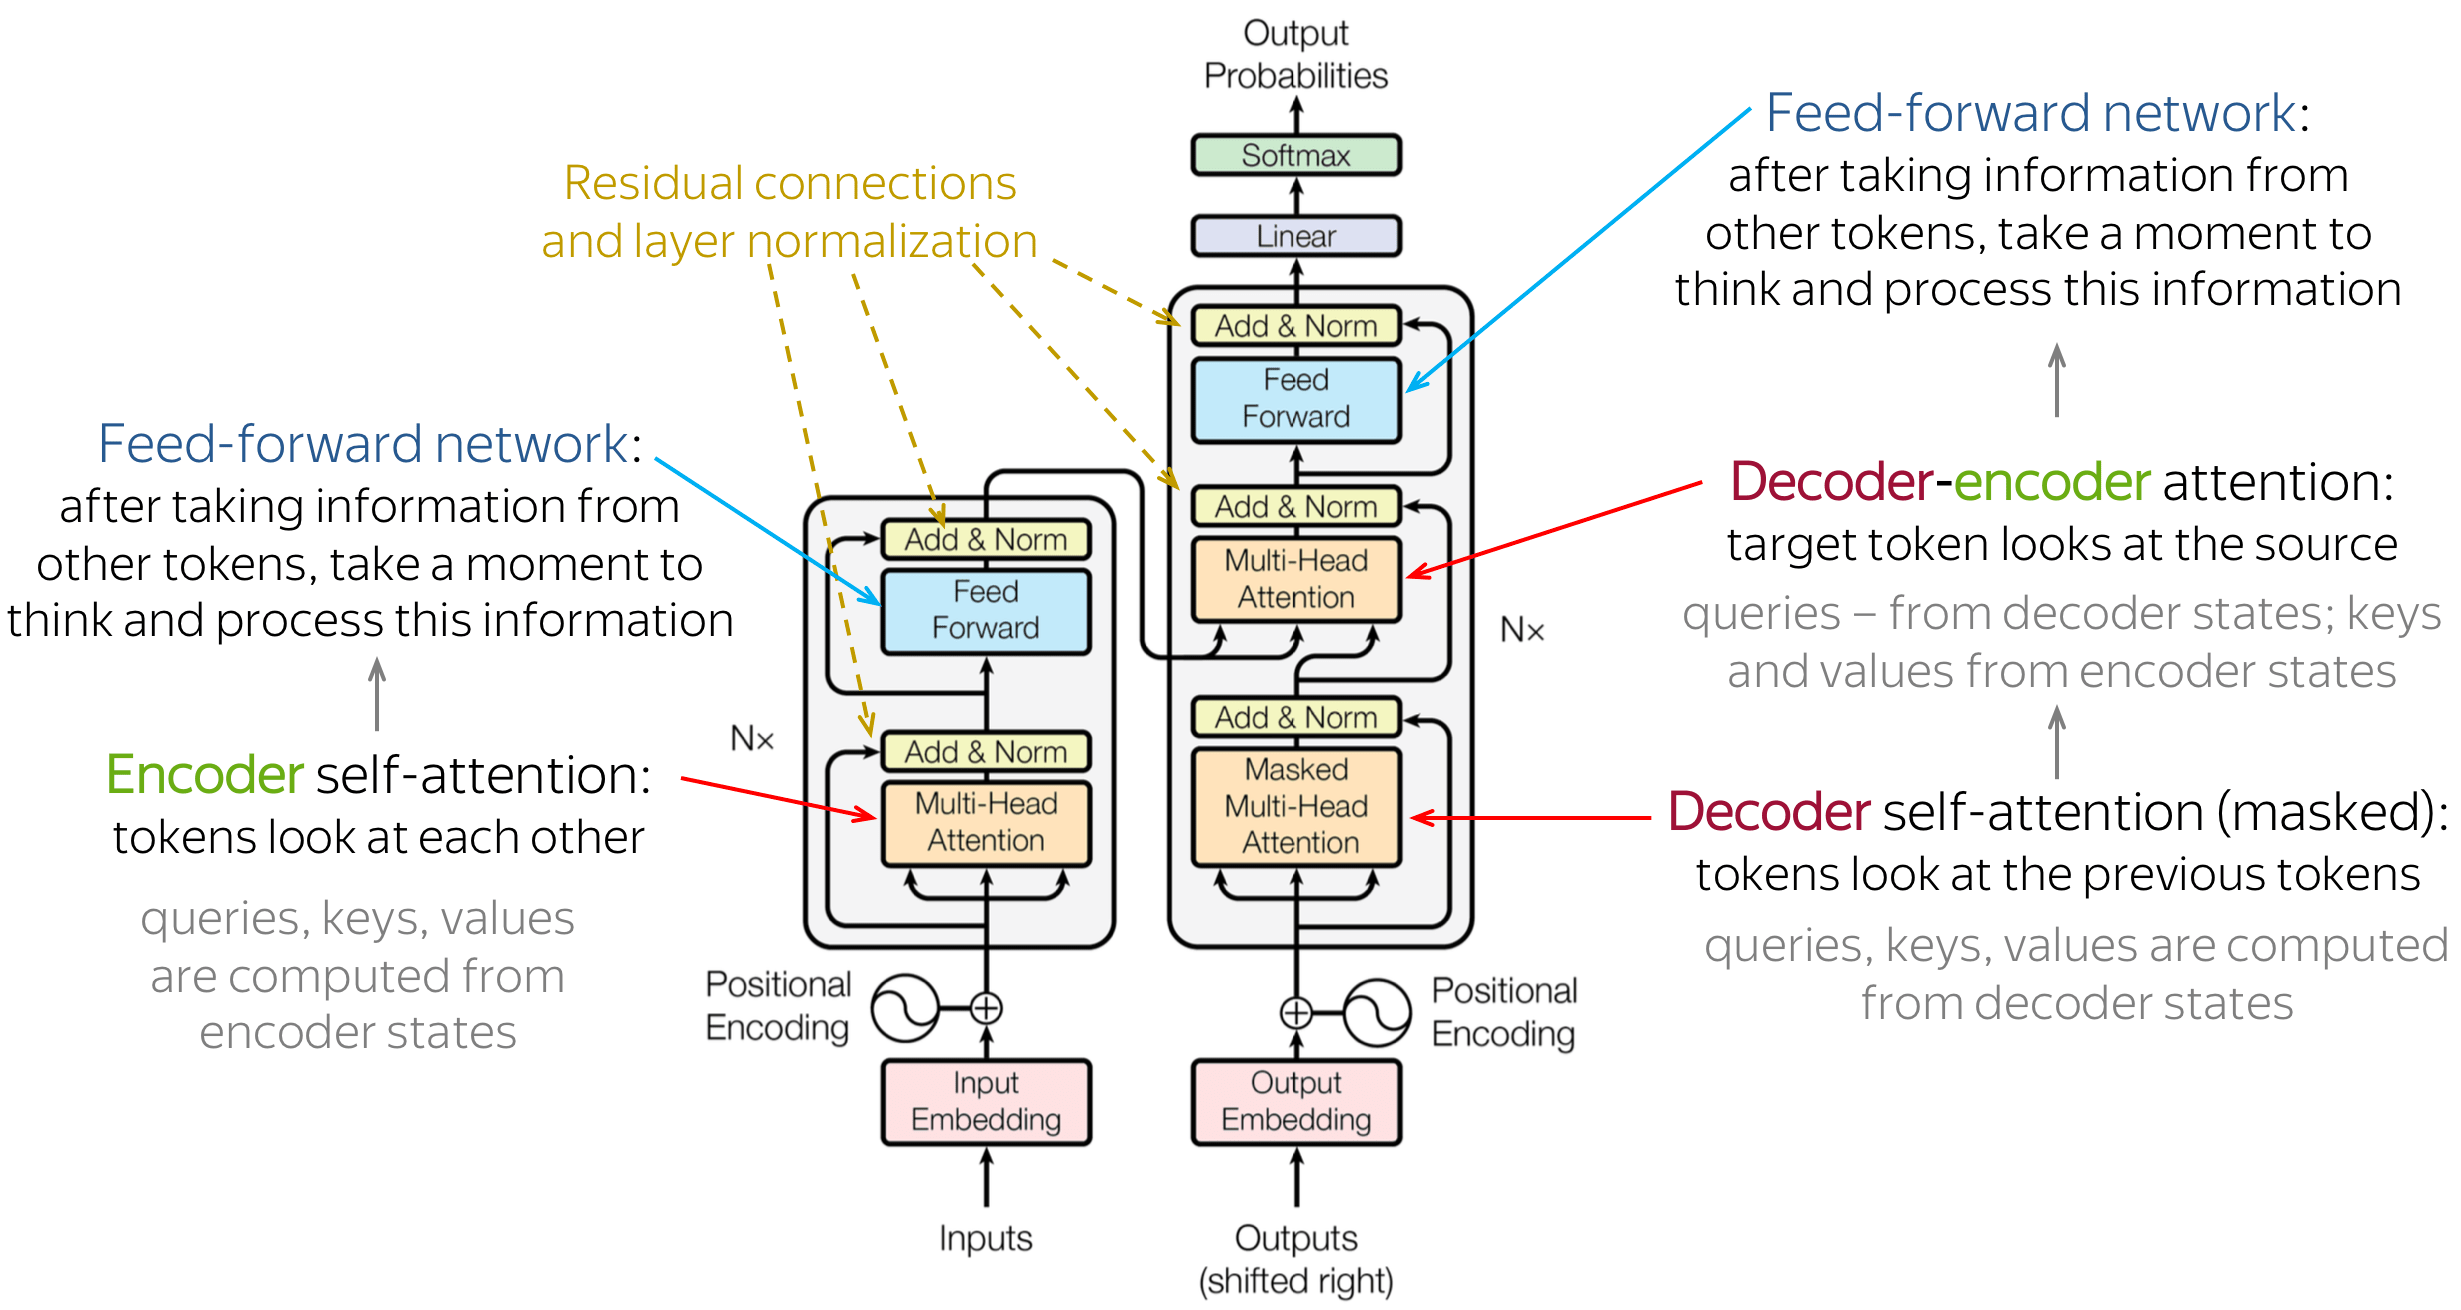
\includegraphics[width=1\linewidth]{f4.png}
        \label{fig:enter-label}
    \end{figure}
    \footnote{image credits: Lena Voita}
\end{frame}

\begin{frame}{Encoder Architecture}
\begin{itemize}
    \item Encoder is made up of 6 identical layers
\end{itemize}
\begin{columns}

  \column{0.25\textwidth}
  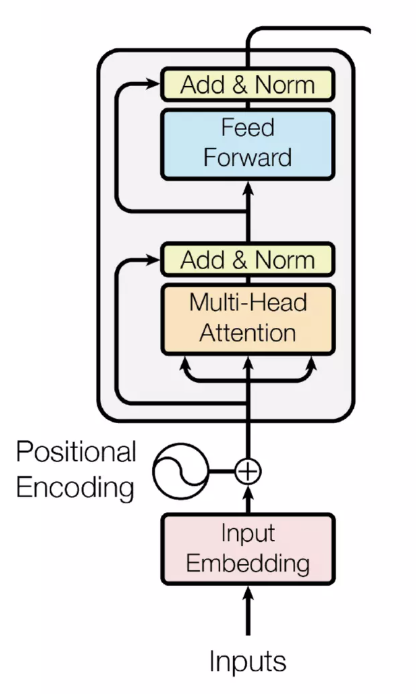
\includegraphics[width=1\linewidth]{f5.png} % Replace with your image filename
  \column{0.75\textwidth}
\begin{itemize}

    \item Each layer has two sub-layers. 
        \begin{itemize}
            \item  First is multi-head self-attention mechanism, 
            \item Second is a simple, position- wise fully connected feed-forward network.
        \end{itemize}
    \item Residual connections\footnote{Kaiming He, Xiangyu Zhang, Shaoqing Ren, and Jian Sun,2016} + Layer Normalizations\footnote{Jimmy Lei Ba, Jamie Ryan Kiros, and Geoffrey E Hinton,2016}.
    \texttt{LayerNorm(x+Sublayer(x))}
    \item To facilitate these residual connections, all sub-layers in the model, as well as the embedding layers, produce outputs of dimension $d_{model} = 512.$
\end{itemize}  
\end{columns}  
\end{frame}

\begin{frame}{Decoder Architecture}

\begin{columns}
  \column{0.25\textwidth}
  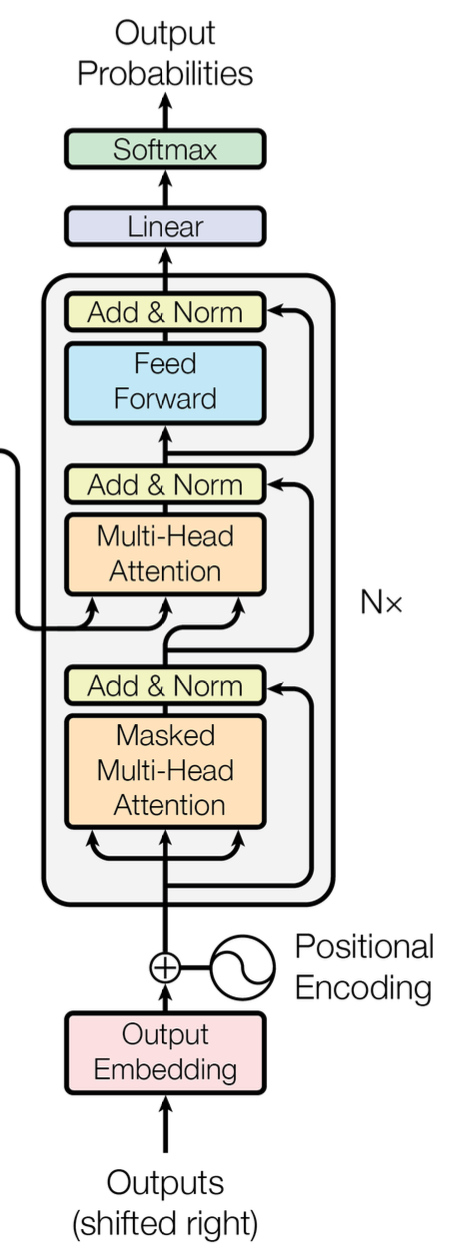
\includegraphics[width=1\linewidth]{f6.png} % Replace with your image filename

  \column{0.75\textwidth}
  \begin{itemize}
      \item The decoder is also composed of a stack of N = 6 identical layers.
      \item In addition to the two sub-layers in each encoder layer, the decoder inserts a third sub-layer, which performs multi-head attention over the output of the encoder stack.
      \item Also modify the self-attention sub-layer in the decoder stack to prevent positions from attending to subsequent positions. 

  \end{itemize}
\end{columns}
\end{frame}

\begin{frame}{Embedding and Positional Encoding.}

\begin{columns}
  \column{0.3\textwidth}
  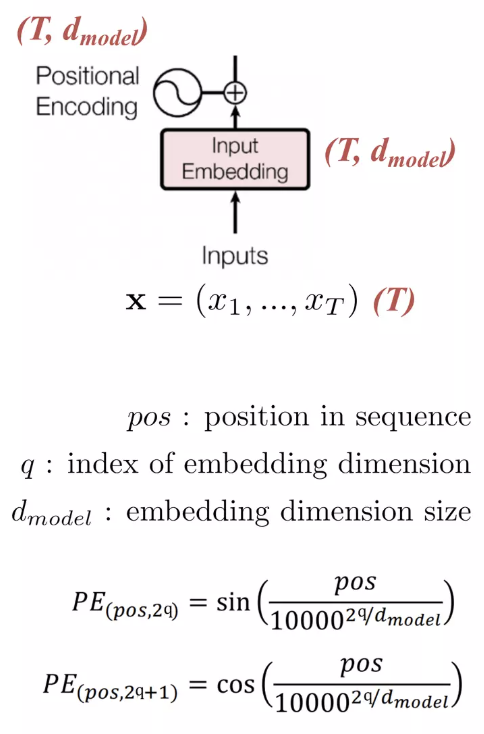
\includegraphics[width=1.25\linewidth]{f7.png} % Replace with your image filename
  \column{0.7\textwidth}
  \begin{itemize}
    \item Transformer does not contain recurrence or convolution, it does not know the order of input tokens.
    \item For this, there are two sets of embeddings: for tokens and for positions(different from rnn).
    \item Then input representation of a token is the sum of two embeddings(both of dimension $d_{model}$)\footnote{Jonas Gehring, Michael Auli, David Grangier, Denis Yarats, and Yann N. Dauphin, 2017.
}
    \item  Each dimension of the positional encoding corresponds to a sinusoid and form a geometric progression from $2\pi$ to $10000\pi$
\end{itemize}
\end{columns}
\end{frame}

\begin{frame}{Attention}
    \begin{itemize}
        \item An attention function can be described as mapping a query and a set of key-value pairs to an output, where the query, keys, values, and output are all vectors. 
        \item The output is computed as a weighted sum of the values, where the weight assigned to each value is computed by a compatibility function of the query with the corresponding key.
        \item The input consists of queries and keys of dimension $d_k$ , and values of dimension $d_v$, divide each by $\sqrt{d_k}$, and apply a softmax function to obtain the weights on the values.
    \end{itemize}
    
    \vspace{0.5em}
    \begin{columns}
        % Left column for formula
        \column{0.45\textwidth}
        \[
        \text{Attention}(Q, K, V) = \text{softmax}\left(\frac{QK^T}{\sqrt{d_k}}\right)V
        \]

        % Right column for image
        \column{0.05\textwidth}
        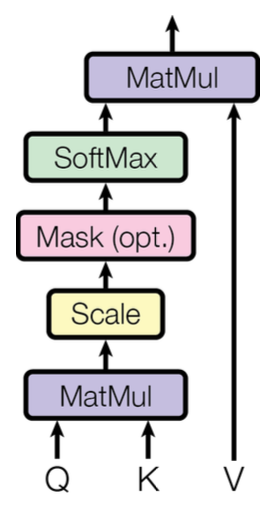
\includegraphics[width=3\linewidth]{f8.png} % Adjust image width if needed
    \end{columns}
\end{frame}

\begin{frame}{Idea behind Attention}

\begin{itemize}
    \item Learn (differentiable) how to pick relevant information from input data.
\end{itemize}

\begin{columns}
    \column{0.4\textwidth}
        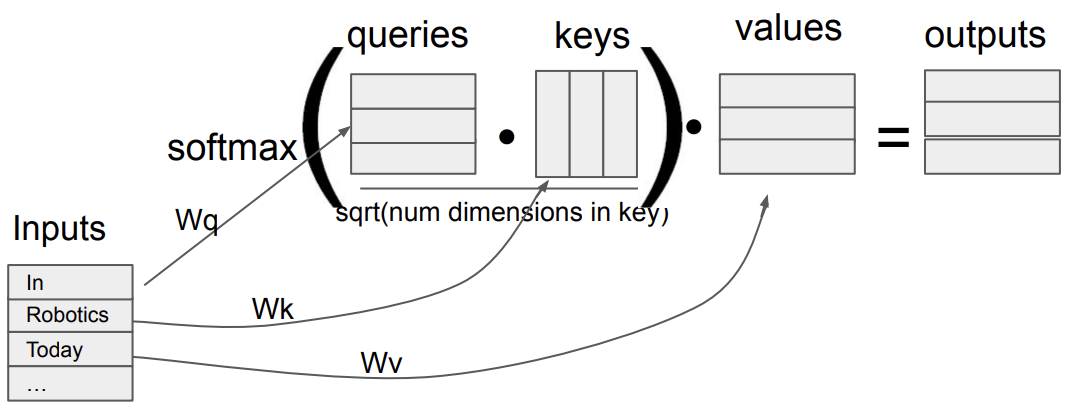
\includegraphics[width=1.2\linewidth]{f9.png} 

    \column{0.6\linewidth}
      \begin{itemize}
        \item Create three vectors from each of the encoder’s input value (query, key, value)
        \item Calculate a score for how much to focus on each part of the input when we encode words at specific positions
        \item Dividing by $d_k$ makes algorithm easier to train
      \end{itemize}
    \end{columns}

\begin{itemize}
    \item The idea is to select a value (referenced by a key) relevant to a query (what trying to pull from input)
\end{itemize}

\end{frame}

\begin{frame}{Idea behind Attention continue...}
    
\end{frame}

\end{document}


